\section{Ubiquitous Language}

\begin{itemize}
    \item \textbf{Aggregate Program}: Specification for a collective behavior that needs to be achieved.
    \item \textbf{Computational Field}: A field is a collective structure that maps each device in some portion of the network to locally computed values over time.
    \item \textbf{Field Calculus}: A programming model in which computational fields are first-class entities.
    \item \textbf{VM}: A Virtual Machine for the execution of an aggregate program.
    \item \textbf{Round}: Correspond to a local computation in a device. Create the context, evaluate the aggregate program and share the exports to the neighborhood.
    \item \textbf{Environment}: An abstraction for the real world.
    \item \textbf{Context}: An abstraction for the local computation's input. It contains the neighbors' exports, the local status of the device and the results of the previous round.
    \item \textbf{Export}: A tree-like data structure that contains all the information needed for coordinating with neighbors and the output of the computation.
    \item \textbf{Network}: A network of heterogeneous devices that act as a collective.
    \item \textbf{Device}: A singular entity that executes the aggregate program. Also called: nodes or agents.
    \item \textbf{Neighboring}: A relation between devices that communicate directly.
    \item \textbf{Sensor}: A physical or virtual component that allows the device to interact with the environment.
    \item \textbf{Abstract Syntax Tree}: A data-oriented representation used by ScaFi to represent the aggregate program structure.
    \item \textbf{Path}: Sequence of slots, corresponding to a branch of the AST.
    \item \textbf{Slot}: A representation for a construct of the language.
    \item \textbf{Language}: The collection of basic constructs.
    \item \textbf{Nbr}: It observes the value of an expression across neighbors, producing a “field of fields”.
    \item \textbf{Rep}: It iteratively updates the value of the input expression at each device using the last computed value.
    \item \textbf{Foldhood}: Aggregates the results of the neighbor computation.
    \item \textbf{Branch}: Partition the domain into two subspaces that do not interact with each other.
    \item \textbf{Alignment}: Two devices are said to be aligned if they have evaluated the same expression and belong to the same domain.
    \item \textbf{Local ID}: It is the ID of the local device.
    \item \textbf{Sense}: Return the value of a local sensor.
    \item \textbf{Exchange}: The exchange construct handles neighbor-to-neighbor propagation of partial accumulates.
    \item \textbf{Share}: Captures the space-time nature of field computation through observation of neighbors’ values, reduction to a single local value and updating and sharing to neighbors of a local variable.
\end{itemize}

\begin{figure}[ht]
    \centering % Centra l'immagine
    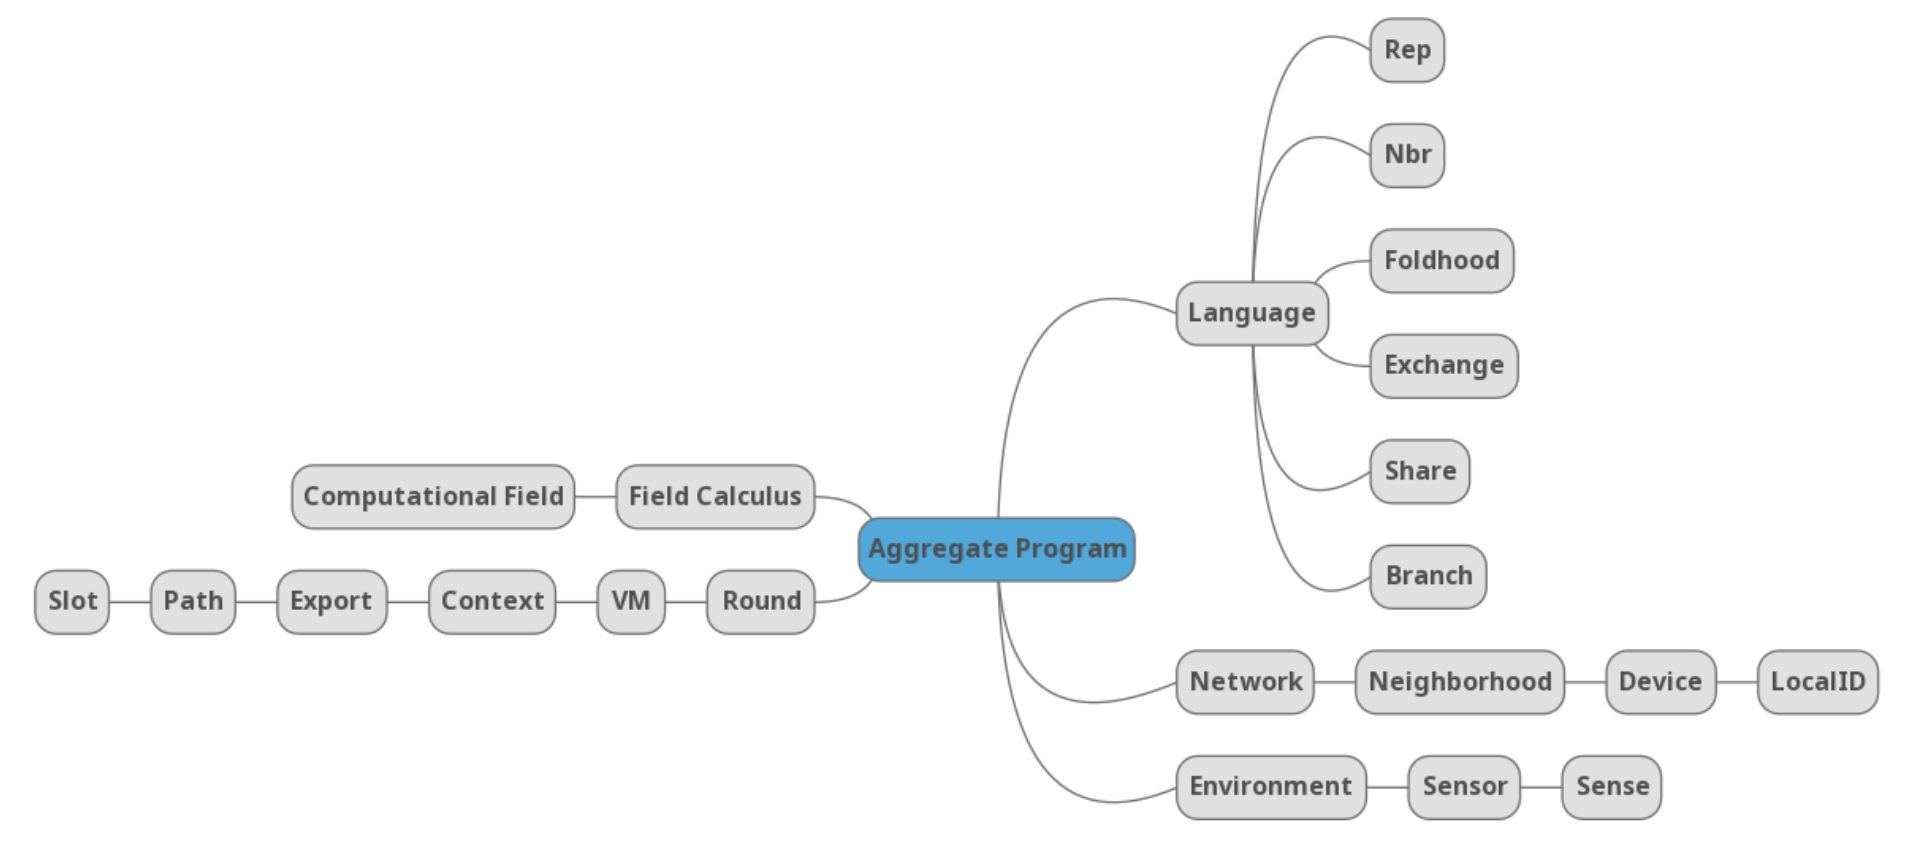
\includegraphics[width=1\linewidth]{images/ul.png}
    \caption{Diagramma dell'Ubiquitous Language}
    \label{fig:ul}
\end{figure}